\section{SPI Interface}
\label{sec:SPI:Interface}

Die \Fachbegriff{Serial Peripheral Interface} (SPI) ist eine der am häufigsten verwendeten Schnittstellen zwischen Mikrocontrollern und Peripherie-ICs wie Sensoren, ADCs, DACs, Schieberegistern, SRAM und anderen. 
Die Schnittstelle SPI ist eine synchrone, auf Voll-Duplex basierte Master-Slave-Schnittstelle. Die Daten vom Master oder Slave werden mit der aufsteigenden oder abfallenden Taktflanke synchronisiert. Dabei können sowohl Master als auch Slave gleichzeitig Daten übertragen. \\
Das SPI arbeitet aber nach dem Single-Master-Prinzip. Das bedeutet, dass ein zentrales Gerät die gesamte Kommunikation mit den Slaves initiiert. Der Master sendet Daten auf der MOSI-Signalleitung und empfängt Daten auf der MISO-Signalleitung, so dass der Busmaster gleichzeitig Daten senden und empfangen kann. wie auf dem Bild A der Abbildung ~\ref{fig:spi:bus} zu sehen ist. Alle Datenübertragungen müssen zwischen dem Bus-Master und den Slaves stattfinden. Datenübertragungen die direkt zwischen zwei Slave-Geräten stattfinden  sind nicht erlaubt. 

\begin{figure}[h]
	\begin{center}
		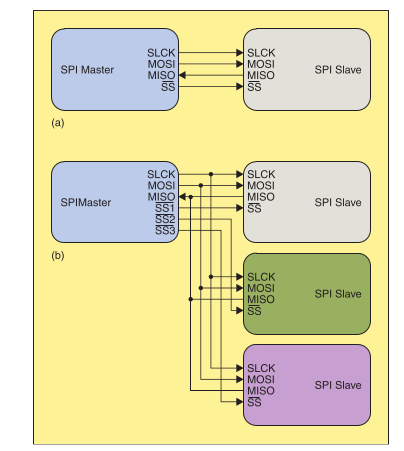
\includegraphics[width=0.8\textwidth]{./images/spi-bus.jpg}
	\end{center}
	\vspace{-5pt}
	\caption[SPI Bus]{SPI Bus \cite{Leens2009}[p.~9]} % Eckige Klammer (optional): Caption-Text in Abbildungsverzeichnis
	\label{fig:spi:bus}
	\vspace{-5pt}
\end{figure}
Möchte der SPI-Master Daten an einen Slave senden und/oder von ihm Informationen anfordern, dann wählt er einen Slave aus, und zwar durch Ziehen der entsprechenden SS-Leitung nach unten, während er das Taktsignal mit einer für den Master und den Slave nutzbaren Taktfrequenz aktiviert.
SPI ist eine Protokoll mit vier Signalleitungen, wie auf \cite{Leens2009}[p.~9] zu lesen ist.
\begin{itemize}
	\item \textbf{Ein Clock-Signal (SCLK)}, welches vom Bus-Master an alle Slaves gesendet wird; alle SPI-Signale sind mit diesem Clock-Signal synchronisiert.
	\item \textbf{Der Slave Select Signal}: der zur Auswahl des Slaves dient, mit dem der Master kommuniziert.
	\item \textbf{Eine Datenleitung vom Master zu den Slaves}, bezeichnet als Master Out-Slave In (MOSI).
	\item \textbf{Eine Datenleitung von den Slaves zum Master}, bezeichnet als Master In-Slave Out (MISO).
\end{itemize}
Im kommenden Abschnitt möchte ich das Thema Embedded Systems ansprechen. und die Vorteile solcher Systeme erläutern. 
%\begin{minipage}{\textwidth}
 % \captionof{lstlisting}[Hello World]{Hello World \cite{coder.2009}} % Eckige Klammer (optional): Caption-Text in Listingsverzeichnis
  %\vspace{-3pt}
  %\begin{lstlisting}[language=java,label=lst:HelloWorld]
%public class HelloWorld
%{
%  public static void main(String[] args)
 % {
  %  System.out.println("HelloWorld");
  %}
%}
%  \end{lstlisting}
%\end{minipage}